It is used to describe the time or space complexity of algorithms. \textbf{Big-O} is a way to express the \textbf{upper bound}, meaning the \textbf{worst case}, of an algorihtm's time or space complexity. Describes the asymptotic behavior (order of growth) of a function, not it's exact value.

The "O" in Big O stands for order, as in order of growth. The letter "O" was chosen by Paul Bachmann to stand for the german word "Ordnung", which means "order". In mathematics, the order of a function refers to how quickly it grows or declines.

\textbf{Big Omega} notation ($\Omega$) defines the \textbf{lower bound}, meaning the \textbf{best case}. \textbf{Big Theta} notation ($\Theta$) describes the exact order of growth, this is the \textbf{tight bound} or \textbf{average case}. Big O is used most of the times.

Time complexity considers two factors, the \textbf{time} ($t$) it takes to complete the task and the \textbf{size} ($n$) of the input.

Fastest to slowest time complexity:

\begin{itemize}
  \item \textbf{Constant:} \textbf{O($1$)}. Time is independent of value of $n$. For example the \sumathsrs.
  \item \textbf{Logarithmic:} \textbf{O($\log n$)} Running time is proportional to the logarithm of $n$. In computing a plain `$\log$' refers to a logarithm of base 2 ($\log_2$). Base 10 ($\log_{10}$) is faster than base 2 ($\log_2$). An example of base 2 is \binarysch.
  \item \textbf{Linear:} \textbf{O($n$)}. Grows linearly with the size of $n$. Single variable loops like \linearsch.
  \item \textbf{Quasilinear:} \textbf{O($n \log n$)}. Running time is proportional to $n$ times the logarithm of $n$. Fastest sorting runtime (e.g. \mergesrt, \heapsrt).
  \item \textbf{Quadratic:} \textbf{O($n^2$)}. Runnig time is porportional to the square of the input size, $n$ times $n$. Traverse square matrix, \bubblesrt, \selectionsrt, \insertionsrt.
  \item \textbf{Exponential:} \textbf{O($2^N$)}. Running time doubles with each addition to $n$. Recursive fibonacci series, levels of a tree.
  \item \textbf{Factorial:} \textbf{O($n!$)}. Running time grows factorially with $n$. This is often seen in algorithms that generate all permutations of a set of data.
\end{itemize}

Plot of time complexity:

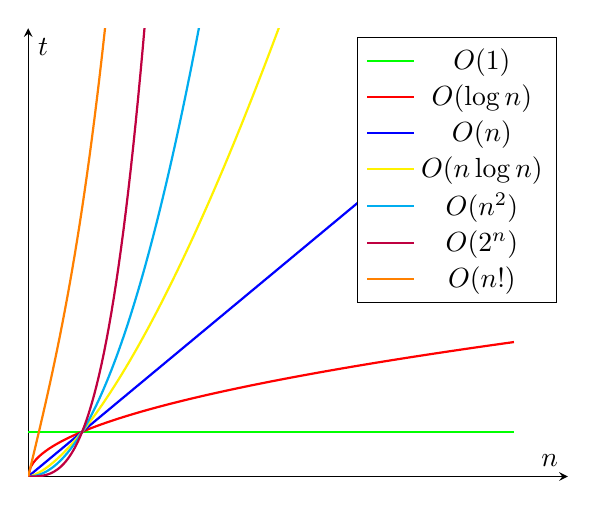
\begin{tikzpicture}[
  declare function={
    log(\b, \x)=ln(\x)/ln(\b);
  }
  ]
  \begin{axis}[
    xmin=0,xmax=10,
    ymin=0,ymax=10,
    xtick={0},ytick={0},
    xlabel={$n$},ylabel={$t$},
    axis lines=center
    ]
    % constant
    \addplot[green,thick,domain=0:9]{1};
    \addlegendentry{$O(1)$}
    % logarithm
    \addplot[red,thick,domain=0:9,samples=200]{x^0.5};
    \addlegendentry{$O(\log n)$}
    % linear
    \addplot[blue,thick,domain=0:9]{x};
    \addlegendentry{$O(n)$}
    % quasilinear
    \addplot[yellow,thick,domain=0:9,samples=200]{x^1.5}; % x * x^0.5
    \addlegendentry{$O(n \log n)$}
    % quadratic
    \addplot[cyan,thick,domain=0:9,samples=200]{x^2};
    \addlegendentry{$O(n^2)$}
    % exponential
    \addplot[purple,thick,domain=0:9,samples=200]{x^3};
    \addlegendentry{$O(2^n)$}
    % factorial
    \addplot[orange,thick,domain=0:9,samples=200]{x^3 + 5*x};
    \addlegendentry{$O(n!)$}
  \end{axis}
\end{tikzpicture}
